As the section before, we want now to show extensions where we split the surface of the triangle mesh likewise into regions around  edges and we draw all pixels in these regions with the same colour (see Figure \ref{fig:edge-area}). This results in rhombus-shaped areas with constant color around each edge.

\begin{figure}[H]
    \centering
    \minipage[b]{.5\linewidth}
    \centering
    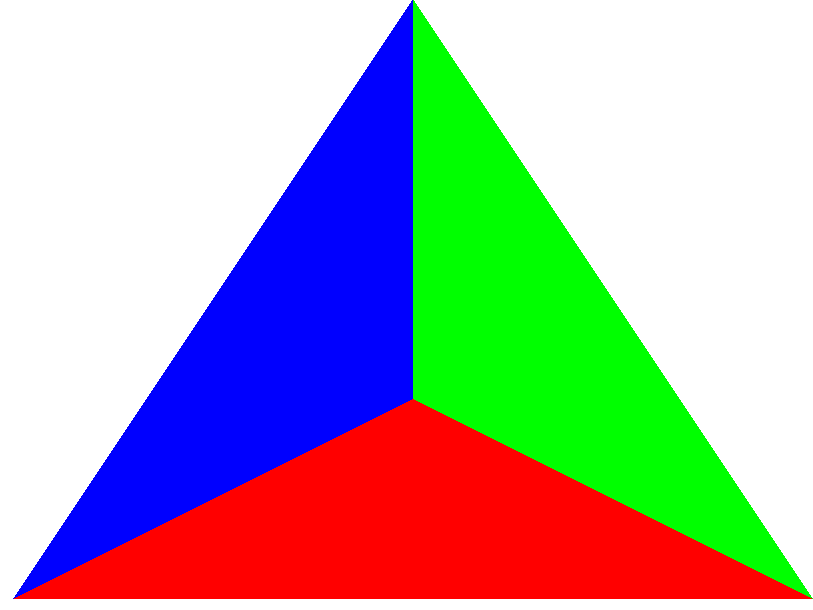
\includegraphics[scale=0.15]{images/min.png}
    \caption{Min diagram}\label{fig:min-diagram}
    \endminipage\hfill
    \minipage[b]{.5\linewidth}
    \centering
    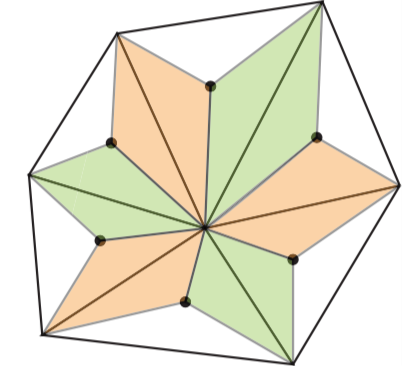
\includegraphics[scale=0.6]{images/edge-area.png}
    \caption{Region around an edge}\label{fig:edge-area}
    \endminipage
\end{figure}

\subsection{Min diagram - Edge based area} \label{section:max-diagram}
For each point in a triangle, we can easily determine its closest edge, which we use as a cue for coloring.
A different approach from interpolating, can be found coloring vertex areas based on the minimum barycentric coordinate.
The color is given by the region farthest from a vertex (Fig. \ref{fig:min-diagram}, Pseudocode \color{red}{insert Pseudocode}\color{black}).

\subsection{Mean Curvature}
Access to mesh edges requires to set up a list of edges over triangles. To avoid redundant datas we have decided to use the convention that an edge would be count only if it goes from a lower to higher vertex. An edge structure contains:
\begin{lstlisting}[caption={Edge structure}]
    struct edge
    {
        float norm_edge;
        int index_v1;
        int index_v2;
        Point3d n1;
        Point3d n2;
        float value_mean_curvature;
        float cot_alpha;
        float cot_beta;
        float area_t1;
        float area_t2;
    };
\end{lstlisting} \label{Pseudocode:edge}

indexes vertices, length of edge, normals of triangles, cotangents of opposite angles to the edge ($\cot \alpha,\; \cot \beta$), areas of triangles. (See edge struct \ref{Pseudocode:edge}).

\subsection{Mean Curvature per edge}
\textit{Mean Curvature per edge} returns a constant color around each edge (See Fig. \ref{fig:armadillo-mean-edge}). It first calculate the mean curvature for each edge:
$$H(E) = || E|| (\theta_E /2)$$
where $\theta_E$ is the angle between the two normals of $T_1$ and $T_2$ (See Fig. \ref{fig:mean-edge}).
\begin{figure}[H]
    \centering
    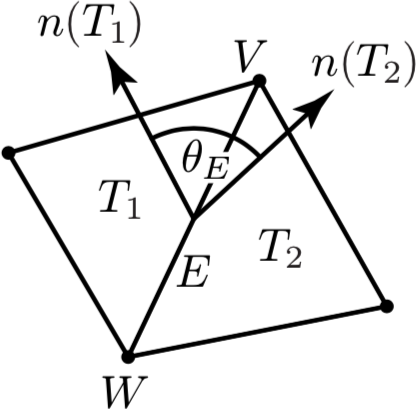
\includegraphics[scale=0.6]{images/mean-edge-theta.png}
    \caption{The dihedral angle $\theta_E$ at a mesh edge $E$ is the angle between the normals of the adjacent triangles. \cite{geometryprocessing}}\label{fig:mean-edge}
\end{figure}
The mean curvature for each vertex $V$ of a mesh is defined as:
$$H(E) = \frac{1}{2\mathcal{A}_{Barycentre}} \sum_{i = 1}^n ||E_i||(\theta_E/2)$$
This value is then normalized since it is an integral value. Every value is then mapped to positive or negative curvature, depending if the mesh at this edge is convex or concave, testing the $3D$ determinant of the 3-by-3 matrix $M = [e, n_1, n_2]$ with those three vectors as
columns ($e$ is the edge $[W, V]$, $n_1$ is the normal of $T_1$ and $n_2$ is the normal of $T_2$). If $det(M) > 0$ then the mesh is convex at $[W, V]$ and the mean curvature would be positive, else the mesh is concave and the mean curvature would be negative. This technique of edge flat shading represents an alternative to the classic triangle flat shading.

\begin{figure}[!h]
    \centering
    \minipage[b]{.5\linewidth}
    \centering
    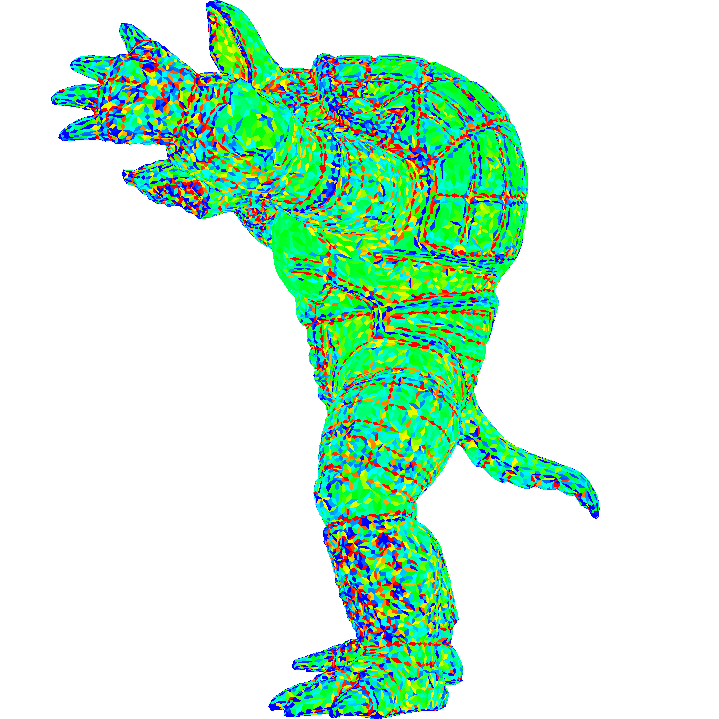
\includegraphics[scale=0.5]{images/mean-curvature-edge.png}
    \endminipage\hfill
    \minipage[b]{.5\linewidth}
    \centering
    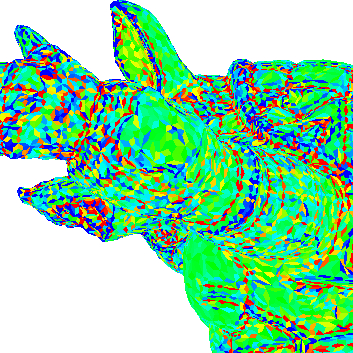
\includegraphics[scale=1.0]{images/mean-curvature-edge-detail.png}
    \endminipage
    \caption{Mean curvature per edge} \label{fig:armadillo-mean-edge}
\end{figure}

\subsection{Mean Curvature per vertex}
\textit{Mean Curvature per vertex} returns an interpolated color around each vertex. The main idea is to calculate the mean curvature $H(V)$ for each vertex $V$. In a mesh, every edge has two opposite angles (let us denominate these with $\alpha$ and $\beta$), the mean curvature per vertex is defined as:
$$H(V) = \frac{1}{2\mathcal{A}_{Mixed}} \sum_{i=1}^{n}(\cot \alpha_i + \cot \beta_i) (V - V_i)$$
where $V_i$ is one of the endpoints of the edge $E_i$ (see Fig. \ref{fig:mean-edge-cot}).
\begin{figure}[H]
    \centering
    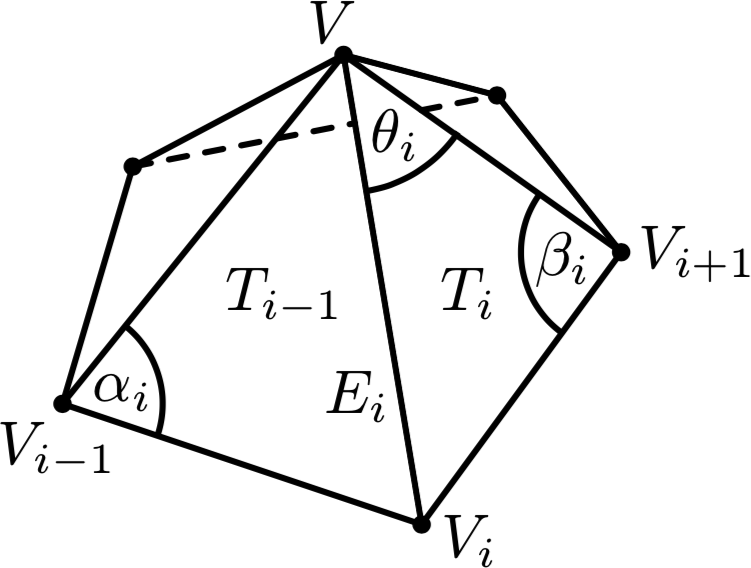
\includegraphics[scale=0.6]{images/mean-edge-cot.png}
    \caption{A vertex $V$ of a triangle mesh with neighbouring vertices $V_i$ and adjacent triangles $T_i$. The angle of $T_i$ at $V$ is denoted by $\theta_i$ and the angles opposite the edge $E_i$ by $\alpha_i$ and $\beta_i$. \cite{geometryprocessing}}\label{fig:mean-edge-cot}
\end{figure}

These values are then interpolated using the automatic OpenGL interpolation resembling the classic Gouraud shading (see Fig. \ref{fig:armadillo-mean-vertex}).

\begin{figure}[!h]
    \centering
    \minipage[b]{.5\linewidth}
    \centering
    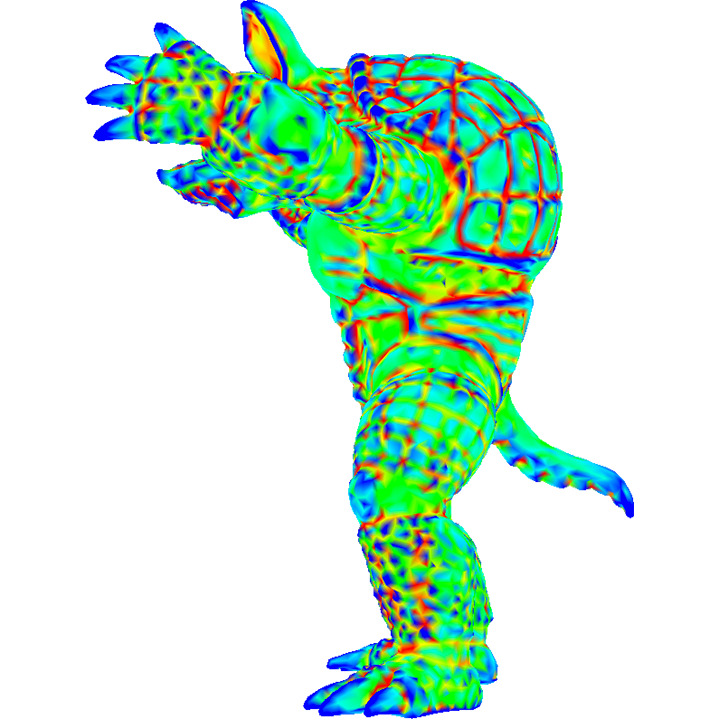
\includegraphics[scale=0.24]{images/mean-curvature-vertex.png}
    \endminipage\hfill
    \minipage[b]{.5\linewidth}
    \centering
    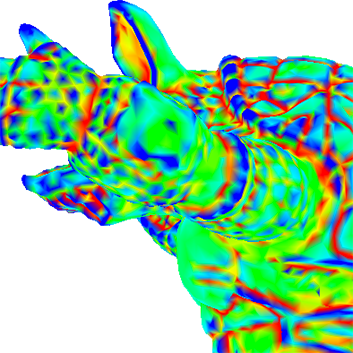
\includegraphics[scale=0.5]{images/mean-curvature-vertex-detail.png}
    \endminipage
    \caption{Mean curvature per vertex} \label{fig:armadillo-mean-vertex}
\end{figure}


\subsection{Evaluation and Comparison between mean curvature per edge and mean curvature per vertex}
list call on Skype
// TODO: image of comparison